\documentclass[12pt]{article}
%\usepackage{polski}
\usepackage{makecell}
\usepackage[colorlinks=true,citecolor=blue,linkcolor=blue, urlcolor=blue]{hyperref}
\usepackage{graphicx}
\usepackage[ruled]{algorithm2e}
\usepackage{algpseudocode}
\usepackage{amsmath}
\setlength\parindent{0pt}
\begin{document}

    \title{Reproduction of SNOW paper \\ \vspace{5mm} \large Deep Learning with Multiple Tasks 2020/2021}
    \author{Wiktor Daniec, Paweł Goliszewski, Konrad Wójtowicz}
    \date{}
    \maketitle


    \section{Introduction}

    Creating models which will be able to handle multiple tasks is current object of research in machine learning field.
    People usually do not need thousands of examples (like many ML model do) to learn how to classify objects into some number of classes of object - they usually use information learned through entire life and adapt quickly to new tasks.
    Idea is to use 'knowledge' from model trained on the other task to learn faster how to manage other task.
    Authors of paper \cite{paper} tackle the problem of image classification.
    They use pretrained model with smaller model connected to it to perform classification task on other classes.
    Our goal was to try to reproduce their results.


    \section{SNOW model architecture}

    This model uses 2 models connected via operation called Channel Pooling which will be described later.
    One model (called source model) is ResNet50 pretrained on ImageNet dataset with frozen weights.
    It is connected after each convolutional layer with second model (called delta model) which is smaller version of Resnet (in our experiments channels reduced by 8) with randomly initialized and trainable weights.
    We put image tensor to both model inputs, and we use only the output of the delta model into consideration.

    \begin{figure}
        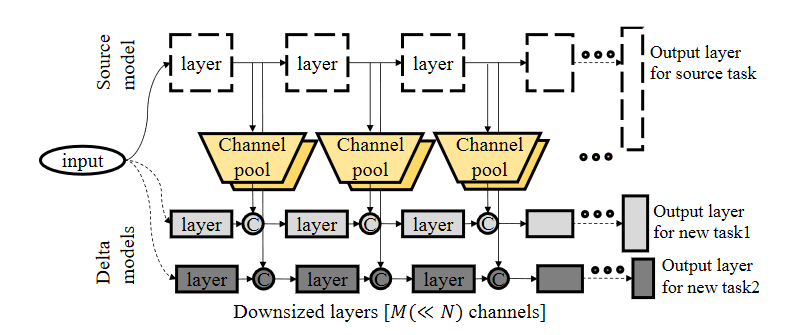
\includegraphics{SNOW.png}
        \caption{Illustration of SNOW model}
    \end{figure}

    \subsection{Channel pooling operation}

    Channel pooling (CP) operation behaves differently during training stage and the evaluation stage.

    CP layer contains weight vector $w$ of size $N$ where $N$ is also number of input tensor layers.
    If it is training time we sample vector size $N$ from normal distribution of mean 0 and standard deviation $\sigma$, and add it to the weights vector obtaining $rand_v$ vector.
    We take indexes of the $M$ biggest values of $rand_v$.
    We take $M$ channels of the input given by those indexes multiplied by $w$ element-wisely.
    We concatenate the result to the corresponding input int the delta model.

    \begin{algorithm}
        $w$: channel pooling weight ($N\times1$ vector)\;
        $x$: input tensor (with $N$ channels)\;
        \SetKwFunction{FMain}{ChannelPoolingFroward}
        \SetKwProg{Pn}{Function}{:}{\KwRet x}
        \Pn{\FMain{$x$}}{
            \eIf{training}{
                $rand_v=w+\mathcal{N}(0,\sigma)$\;
                $\_,idx=\text{topK}(rand_v,M)$\;
                $selected\_weights=w[idx]$
            }{
                $selected\_weights,idx=\text{topK}(rand_v,M)$\;
            }
            \EndIf
            $x = x[idx]$\;
            $x = x \bigotimes selected\_weights$\;
        }
        \caption{Channel Pooling pseudocode}\label{alg:algorithm}
    \end{algorithm}


    \section{Transfer learning}

    We use some standard transfer learning techniques for comparison.
    Those techniques are:
    \begin{itemize}
        \item full fine-tuning (FT) - We use pretrained ResNet50, and we modify last layer to adjust number of classes to a new task. Then we train network with all trainable parameters on a new task.
        \item feature extraction (FE) - Similarly as above, but weights of first 3 bottlenecks are frozen.
        \item final layer only (FO) - Similarly as above, but only last linear layer is not frozen.
    \end{itemize}

    \section{Experiments}

    \subsection{Datasets}

    We used 5 datasets: Action, Cars, DTD, Birds, Food-101.

    Action dataset contains 9532 images (4000 in training dataset and 5532 in the test dataset) divided into 40 classes.
    Images contain

    \subsection{Transfer learning}

    \subsection{SNOW}

    \subsection{Throughput}

    \subsection{Visualization of filters}


    \section{Conslusions}

    \begin{thebibliography}{99}
        \bibitem{paper} \href{https://openreview.net/pdf?id=rJxtgJBKDr}{https://openreview.net/pdf?id=rJxtgJBKDr} \\
        Chungkuk Yoo, Bumsoo Kang, Minsik Cho, SNOW: Subscribing to Knowledge via Channel Pooling for Transfer \& Lifelong Learning of Convolutional Neural Networks, ICLR 2020
    \end{thebibliography}
\end{document}
